%==========================================================================
% XSS Sentinel: Contextual-Adversarial Cross-Feature (CAXF) Extraction with
% TF-IDF N-Grams, Character-Level CNN, and MiniLM Sentence Embeddings
% for Multi-Class XSS Detection via Six Heterogeneous Ensemble Strategies
%
% Custom Section Format (plain article, NOT IEEE/ACM/Springer template)
% Compile: pdflatex -> bibtex -> pdflatex -> pdflatex
%==========================================================================
\documentclass[11pt,a4paper]{article}

\usepackage[margin=2.5cm]{geometry}
\usepackage{amsmath,amssymb,amsfonts}
\usepackage{algorithmic}
\usepackage{algorithm}
\usepackage{graphicx}
\usepackage{textcomp}
\usepackage{xcolor}
\usepackage{booktabs}
\usepackage{multirow}
\usepackage{url}
\usepackage{cite}
\usepackage{setspace}
\usepackage{titlesec}
\usepackage{hyperref}
\usepackage{parskip}
\usepackage{subcaption}
\usepackage{tikz}
\usetikzlibrary{arrows.meta, shapes.geometric, positioning, fit, backgrounds}

\onehalfspacing

\hypersetup{
  colorlinks=true,
  linkcolor=blue!60!black,
  citecolor=blue!60!black,
  urlcolor=blue!60!black
}

\titleformat{\section}{\large\bfseries}{\thesection.}{0.6em}{}
\titleformat{\subsection}{\normalsize\bfseries}{\thesubsection}{0.5em}{}
\titleformat{\subsubsection}{\normalsize\itshape}{\thesubsubsection}{0.4em}{}

%==========================================================================
\begin{document}

%--------------------------------------------------------------------------
%  PAGE 1 - TITLE AND AUTHORS
%--------------------------------------------------------------------------

\begin{center}
  {\LARGE\bfseries
   XSS Sentinel: Contextual-Adversarial Cross-Feature (CAXF) Extraction and heterogeneous ensemble decision strategies for Multi-Class XSS Detection}
  \vspace{1em}

  {\large Bharathi Sathyan, Mirudhulabashini N}

  % TODO: author details -- affiliations, emails, department, institution, city, country

  \vspace{0.5em}
  \hrule height 0.6pt
\end{center}

\vspace{1em}

%--------------------------------------------------------------------------
%  ABSTRACT
%--------------------------------------------------------------------------

\begin{abstract}
\noindent
Cross-Site Scripting (XSS) is one of the most persistently exploited web attack vectors, yet
fine-grained multi-class XSS classification---distinguishing Reflected, Stored, and DOM-based XSS
from benign payloads---remains underexplored due to severe class imbalance and payload obfuscation.
This paper proposes \textbf{XSS Sentinel}, a framework that combines the
Contextual-Adversarial Cross-Feature (CAXF) extraction pipeline with six heterogeneous
ensemble decision strategies evaluated across three feature representations.
The novelty lies in a structured six-component CAXF feature concatenation covering HTML-structural,
JavaScript-event, URL-pattern, special-character, keyword, and deep-embedding features; a reimplemented
\textit{Strict LCCDE} using out-of-fold (OOF) cross-validation for class-leader identification instead
of heuristic selection; and four novel ensemble strategies---Weighted Soft Voting (WSV), Bayesian Model
Averaging (BMA), Per-Class Expert Routing (PCER), and Confidence-Calibrated Dynamic Selection
(CCDS)---alongside Stacking with a logistic-regression meta-learner.
Experiments are conducted on a publicly available Kaggle XSS dataset comprising 10,917 payloads
across four classes: Normal (3,594), Reflected XSS (6,795), Stored XSS (498), and DOM-based XSS (30).
A 70:30 stratified split (seed=42) yields 7,641 training and 3,276 test samples; SMOTE balances all
training classes to 4,756 samples each. Three CAXF instantiations are evaluated: TF-IDF character
n-gram (5,282-dim), Character-level CNN (410-dim), and all-MiniLM-L6-v2 sentence embedding (666-dim),
with evaluation metrics including macro-averaged Precision, Recall, and F1-score. Stacking with
CAXF+TF-IDF achieves the best macro-F1 of 95.30\% at 99.69\% accuracy; BMA/PCER/WSV with
CAXF+Sentence Embedding achieve macro-precision of 99.29\% and macro-F1 of 95.98\%. An ablation
confirms that Strict LCCDE outperforms the MVE-CT variant on TF-IDF by 1.09 percentage points;
all five proposed ensembles outperform LCCDE on at least one feature representation, compared against
LCCDE~\cite{lccde2022}, MVE-CT~\cite{caxf_lccde2024}, and standalone LightGBM, XGBoost, and CatBoost baselines.
\end{abstract}

\textbf{Keywords:} Cross-Site Scripting, XSS detection, multi-class classification,
ensemble learning, CAXF, LCCDE, character n-gram, CharCNN, sentence embeddings, imbalanced classification.

\vspace{1em}
\hrule height 0.4pt
\vspace{1em}

%==========================================================================
\section{Introduction}
\label{sec:intro}
%==========================================================================

Cross-Site Scripting (XSS) is consistently listed among the top web security
threats by OWASP~\cite{owasp2021}. An XSS attack injects malicious scripts into
trusted web pages, potentially enabling session hijacking, credential theft,
phishing, and client-side malware execution. XSS attacks are broadly
categorized into three primary variants: Reflected XSS, Stored XSS, and
DOM-based XSS. The characteristics and execution mechanisms of these three
attack types, along with their implications for detection, are discussed in
detail in Section~2.1. Accurately classifying an XSS payload into one of
these categories is critical for targeted remediation and WAF rule construction, yet most detection
systems treat XSS as a binary problem.

Three technical challenges dominate the field. Payload obfuscation is the first: attackers encode
scripts via HTML entity encoding, Unicode escaping, JavaScript string splitting, and character
substitution, defeating token-level pattern matching. The second is severe class imbalance, as
DOM-based XSS constitutes fewer than 0.3\% of realistic datasets (30 out of 10,917 samples in this
work), making standard classifier training unreliable without explicit mitigation. The third is
categorical diversity, since the structural and semantic differences among XSS variants require feature
representations that simultaneously capture syntactic, structural, and semantic information.

Prior work on XSS detection largely relies on binary classification using shallow TF-IDF
features~\cite{caxf_lccde2024} or signature-based methods that fail against polymorphic payloads.
The CAXF-LCCDE framework~\cite{caxf_lccde2024} introduced a structured feature concatenation
architecture and the Leader-Confidence-Class Decision Ensemble (LCCDE). However, three limitations
remain: class leaders are assigned heuristically rather than via cross-validation; the framework was
not systematically evaluated for multi-class XSS discrimination across multiple feature spaces; and
probabilistic ensemble alternatives have not been explored.

This paper makes five contributions. First, it introduces a multi-class CAXF pipeline with three
deep-embedding backends: TF-IDF character n-grams, a Character-level CNN (CharCNN), and
all-MiniLM-L6-v2 sentence embeddings. Second, it presents \textit{Strict LCCDE}, a reimplementation
of the LCCDE algorithm using 3-fold OOF cross-validation for data-driven class-leader identification.
Third, it proposes four novel ensemble strategies: Weighted Soft Voting (WSV), Bayesian Model
Averaging (BMA), Per-Class Expert Routing (PCER), and Confidence-Calibrated Dynamic Selection (CCDS).
Fourth, it contributes a Stacking ensemble with a logistic-regression meta-learner trained on 5-fold
OOF features. Fifth, it provides a systematic ablation comparing Strict LCCDE vs.\ MVE-CT across all
three feature representations.

The remainder of this paper is organised as follows. Section~\ref{sec:prelim} establishes the theoretical background, covering XSS attack taxonomy, feature representation strategies for web payloads, gradient-boosting classifiers, and class-imbalance mitigation via SMOTE. Section~\ref{sec:related} surveys related work in XSS detection, ensemble learning for cybersecurity, and imbalanced classification. Section~\ref{sec:problem} formally states the problem, specifying the inputs, constraints, and objectives. Section~\ref{sec:proposed} presents the proposed XSS Sentinel framework in full, describing data collection, preprocessing, model construction, and the complete experimental evaluation---including setup, quantitative results, findings, and the pipeline architecture diagram. Section~\ref{sec:conclusion} summarises the conclusions, discusses the pros and limitations of the approach, and Section~\ref{sec:future} outlines directions for future work.

%==========================================================================
\section{Preliminaries / Background}
\label{sec:prelim}
%==========================================================================

This section establishes the theoretical foundations underlying XSS Sentinel. Understanding the
taxonomy of XSS attacks, the range of applicable feature representations for textual payloads, the
behaviour of gradient-boosting classifiers used as base learners, and the mechanics of class-imbalance
mitigation is essential for interpreting the design choices and experimental results presented in
subsequent sections.

\subsection{Cross-Site Scripting Attack Types}

From a detection perspective, the three XSS categories differ primarily in how
attacker-controlled data reaches the browser and how the malicious content is
delivered. Reflected XSS is associated with request--response interactions,
whereas Stored XSS introduces a persistence component because the malicious
content remains available after the original submission. DOM-based XSS shifts
the execution process entirely to the client side, relying on browser-side
JavaScript and attacker-controlled DOM sources.

These differences have direct implications for feature extraction and
classification. Reflected and Stored XSS can exhibit server- or
request-related characteristics that can be represented through URL,
HTML, JavaScript-event, and keyword features. In contrast, DOM-based XSS may
not produce a distinctive server-side interaction because its execution can
occur without a server round-trip. Consequently, identifying this category
requires features capable of capturing client-side structural and syntactic
patterns within the payload itself. This distinction motivates the use of
multiple complementary feature representations in XSS Sentinel, allowing
structural, character-level, and semantic characteristics of payloads to be
considered jointly.

\subsection{Feature Representation for Web Payloads}

Textual web payloads can be represented at multiple granularities, each capturing a different aspect
of attack intent. Structural features---including HTML tag occurrence counts extracted by BeautifulSoup,
JavaScript event handler frequencies such as \texttt{onerror} and \texttt{onload}, URL structural
attributes, and special-character frequency vectors---capture the syntactic shape of a payload at the
parse-tree level and remain stable under common obfuscation transforms like HTML entity encoding.
Character n-gram TF-IDF applies Term Frequency--Inverse Document Frequency to sub-word units,
detecting patterns such as \texttt{<sc} and \texttt{ript>} that survive partial obfuscation and cannot
be blocked by simple keyword filtering. Character-level CNN models apply convolutional filters directly
to raw character sequences without word tokenisation, capturing positional n-gram patterns in a
distributed, trainable manner. Transformer-based sentence embeddings, produced by models such as
all-MiniLM-L6-v2~\cite{minilm2020}, generate dense fixed-length vectors via mean-pooling over final
hidden states, capturing semantic similarity that is invariant to token-level substitutions.

\subsection{Gradient-Boosting Classifiers}

Three gradient-boosting algorithms serve as base classifiers in this work. LightGBM employs
leaf-wise tree growth with histogram-based splitting, minimising cross-entropy loss and training in
12 to 156 seconds depending on feature dimensionality. XGBoost uses regularised boosting with
second-order gradient statistics~\cite{xgboost2016}, with training times ranging from 19 to 284
seconds. CatBoost applies symmetric-tree boosting with a class-weighted loss, where weights
$w_c = N/(C \cdot N_c)$ yield $w_{\text{DOM}} \approx 90.96$, $w_{\text{Stored}} \approx 5.47$,
$w_{\text{Normal}} \approx 0.76$, and $w_{\text{Reflected}} \approx 0.40$, training in 21 to 521
seconds. These three classifiers are chosen for their complementary inductive biases: LightGBM is
fast and high-recall; XGBoost provides regularisation-controlled precision; CatBoost is
imbalance-aware through its loss-function weighting scheme.

\subsection{Class Imbalance and SMOTE}

SMOTE~\cite{smote2002} addresses class imbalance by generating synthetic minority-class samples
through linear interpolation in feature space. Specifically, given a minority-class sample
$\mathbf{x}_i$ and one of its $k$-nearest neighbours $\mathbf{x}_j$, a synthetic sample is computed
as:
\begin{equation}
  \mathbf{x}_{\text{syn}} = \mathbf{x}_i + \lambda (\mathbf{x}_j - \mathbf{x}_i),
  \quad \lambda \sim \mathcal{U}(0,1)
  \label{eq:smote}
\end{equation}
In this dataset the pre-SMOTE training distribution (DOM=21, Normal=2,515, Reflected=4,756,
Stored=349) is up-sampled uniformly to 4,756 samples per class, yielding 19,024 balanced training
examples. For CatBoost, the same class-weighting formula is applied in the loss function rather than
oversampling, providing a complementary implicit balancing strategy.

%==========================================================================
\section{Related Works}
\label{sec:related}
%==========================================================================

The literature on XSS detection spans classical rule-based systems, machine learning approaches, deep
learning architectures, and ensemble methods. This section surveys the most directly relevant work
across these areas and identifies the gaps that motivate the contributions of XSS Sentinel.

\subsection{XSS Detection Methods}

Early XSS detectors relied on signature matching and regular expressions. While computationally
efficient, these methods fundamentally fail against polymorphic payloads: an attacker who adds a
single character of encoding or splits a keyword across concatenation operations can trivially
evade any finite rule set~\cite{lccde2022}. Machine learning approaches using bag-of-words or TF-IDF
features showed meaningful improvements over rule-based systems but lack structural context derived
from the HTML parse tree or JavaScript event model. The CAXF-LCCDE framework~\cite{caxf_lccde2024}
addressed structural context by concatenating five engineered feature extractors into a unified vector,
demonstrating strong binary XSS-vs.-benign detection; however, multi-class fine-grained classification
and the evaluation of alternative feature backends were not explored. Character-level CNN
models~\cite{charcnn_zhang2015} operate directly on raw character sequences and are therefore
inherently robust to token-level obfuscation, capturing sub-word patterns that persist through
encoding transforms. Transformer-based sentence embeddings (MiniLM)~\cite{minilm2020} represent the
semantic content of payloads in a continuous 384-dimensional space, enabling similarity-based
reasoning that is robust to surface-form variation.

\subsection{Ensemble Learning for Cybersecurity}

LCCDE~\cite{lccde2022} demonstrated that heterogeneous gradient-boosting ensembles substantially
outperform single models for network intrusion detection by assigning prediction authority to the
empirically strongest model for each class. The key innovation was the class-leader concept: rather
than averaging all models equally, each class delegates to its best-performing classifier. Stacking
(Wolpert, 1992)~\cite{wolpert1992} generalises this idea by replacing hand-coded delegation rules
with a meta-learner trained on out-of-fold predictions, enabling the ensemble to learn complex
correlations among base-classifier confidence distributions. Bayesian Model Averaging~\cite{hoeting1999}
provides a principled probabilistic framework for model combination, computing posterior model weights
from class-level precision scores. For severely imbalanced data---such as the DOM-based XSS class in
this work---per-class routing strategies, as embodied in PCER, improve rare-class detection by
directing each test sample to the specialist classifier most qualified for the most-likely predicted
category.

\subsection{Imbalanced Classification in Security}

SMOTE~\cite{smote2002} is the most widely applied oversampling technique in intrusion detection,
malware classification, and fraud detection, where class imbalance ratios often exceed 100:1. For XSS
datasets, DOM-based XSS with only 30 original samples poses extreme challenges: SMOTE generates
4,735 synthetic DOM-based samples, but their diversity is fundamentally limited by the small
neighbourhood structure of 21 training exemplars. CatBoost class-weighting provides a complementary
strategy that operates in the loss-function space rather than the data space, amplifying gradient
signals from rare-class misclassifications without the risk of SMOTE-induced overfitting to
synthetic near-duplicates. Combining both strategies---SMOTE for LightGBM and XGBoost, class
weights for CatBoost---within a single heterogeneous ensemble offers a principled hedge against
the limitations of either approach alone.

%==========================================================================
\section{Problem Statement}
\label{sec:problem}
%==========================================================================

This section formally specifies the inputs available to the system, the constraints under which
it operates, and the precise objectives it must satisfy. A clear problem statement is necessary to
distinguish this work from binary XSS detection, to justify the design of the CAXF pipeline, and to
define the experimental evaluation criteria used in Section~\ref{sec:proposed}.

\subsection{Given (Inputs and Assumptions)}

The system is provided with a corpus of web payloads
$\mathcal{S} = \{(s_i, y_i)\}_{i=1}^{N}$, where each payload $s_i$ is a
raw text string (an HTML/JavaScript/URL fragment) and
$y_i \in \mathcal{C}$ where $C = \{\text{DOM-based XSS}, \text{Normal},
\text{Reflected XSS}, \text{Stored XSS}\}$ is a four-class label.
The dataset used throughout this work comprises $N = 10{,}917$ samples,
with the following class distribution: Normal (3,594), Reflected XSS
(6,795), Stored XSS (498), and DOM-based XSS (30). The data is
partitioned using a 70:30 stratified split with random seed $42$,
yielding 7,641 training samples and 3,276 test samples; zero train-test
overlap is verified programmatically at runtime. A critical operating
constraint is the severe class imbalance. DOM-based XSS constitutes
only 0.27\% of all samples and has a test support of only 9 samples,
making its detection particularly challenging.

\subsection{Objective}

The objective of this work is to construct a multi-class classification model using structured feature
extraction using CAXF (Contextual Adversarial Cross-Feature Extraction) with TF-IDF N-Grams, Character-Level CNN, and MiniLM Sentence Embeddings and heterogeneous ensemble decision strategies, targeting four simultaneous goals. The first
is to accurately classify each web payload into one of the four XSS categories with special emphasis on
rare-class detection for DOM-based and Stored XSS, where misclassifications carry the highest security
cost. The second is to evaluate three CAXF feature representations---character n-gram TF-IDF, Character-
level CNN, and MiniLM sentence embeddings---and determine which feature space best supports each
ensemble strategy, rather than committing to a single representation. The third is to systematically
compare six ensemble decision strategies (Strict LCCDE, WSV, BMA, Stacking, PCER, CCDS) against
the LCCDE baseline and individual base classifiers across all three feature spaces, using macro-averaged
Precision, Recall, and F1-score as primary evaluation metrics. The fourth is to conduct an ablation
study that validates whether OOF-based class-leader identification (Strict LCCDE) statistically
improves upon the heuristic MVE-CT variant proposed in the base paper~\cite{caxf_lccde2024}.

%==========================================================================
\section{Proposed Work}
\label{sec:proposed}
%==========================================================================

XSS Sentinel is built as a modular five-stage pipeline: data collection, preprocessing, model
construction, and then a comprehensive experimental evaluation that includes controlled setup,
quantitative results, interpretive findings, and a visual summary of the architecture. Each stage
is described in detail in the following subsections. The pipeline is designed so that swapping the
feature extraction backend---from TF-IDF to CharCNN to SentEmb---requires only an import-level
change, keeping all downstream ensemble code identical across the three experimental conditions.

%--------------------------------------------------------------------------
\subsection{Data Collection}
\label{ssec:data}
%--------------------------------------------------------------------------

The dataset used in this work is the \textbf{Kaggle XSS Dataset}~\cite{kaggle_xss}, a publicly
available four-class benchmark. Each record is
a raw text string representing a web payload, annotated with one of four class labels. The full
dataset contains 10,917 payloads with the following class-level distribution confirmed from
runtime logs: Reflected XSS accounts for 6,795 samples (62.2\%), Normal for 3,594 (32.9\%), Stored
XSS for 498 (4.6\%), and DOM-based XSS for just 30 samples (0.3\%). Stratified splitting at a 70:30
ratio with seed=42 yields 7,641 training samples and 3,276 test samples, preserving the class
proportions in both subsets. The test-set support per class is: DOM-based XSS (9), Normal (1,079),
Reflected XSS (2,039), and Stored XSS (149). Zero overlap between training and test partitions is
verified programmatically at the start of every experiment run. Table~\ref{tab:dataset} presents
the complete class-wise split statistics.

\begin{table}[ht]
\centering
\caption{Dataset class distribution: full corpus and stratified 70:30 split (seed=42)}
\label{tab:dataset}
\begin{tabular}{lrrrr}
\toprule
\textbf{Class} & \textbf{Total} & \textbf{Train (70\%)} & \textbf{Test (30\%)} & \textbf{\% Total} \\
\midrule
Reflected XSS  & 6,795 & 4,756 & 2,039 & 62.2\% \\
Normal         & 3,594 & 2,515 & 1,079 & 32.9\% \\
Stored XSS     &   498 &   349 &   149 &  4.6\% \\
DOM-based XSS  &    30 &    21 &     9 &  0.3\% \\
\midrule
\textbf{Total} & \textbf{10,917} & \textbf{7,641} & \textbf{3,276} & 100\% \\
\bottomrule
\end{tabular}
\end{table}

%--------------------------------------------------------------------------
\subsection{Preprocessing}
\label{ssec:preproc}
%--------------------------------------------------------------------------

Preprocessing in XSS Sentinel operates at two complementary levels: structural parsing of the raw
payload text into engineered feature sub-vectors, and deep-embedding encoding that maps each payload
into a dense representation learned by a neural model. The five structural sub-extractors are shared
across all three CAXF variants and produce 282 common features; only the deep-embedding component
changes between the TF-IDF, CharCNN, and MiniLM instantiations.

\subsubsection{Structural Sub-Extractors}

The HTML Tags extractor uses BeautifulSoup to parse each payload and count
occurrences of each HTML tag in a fixed vocabulary. The JS Events extractor  computes frequency counts of JavaScript event handler keywords such as \texttt{onerror},
\texttt{onload}, and \texttt{onclick}. The URL Features extractor 
produces binary and count-based encodings of URL structural attributes, including scheme presence,
path depth, query parameter count, and fragment indicator. The Special Characters extractor
 records frequency counts of characters that are particularly significant
for XSS payloads, namely \texttt{<}, \texttt{>}, \texttt{/}, \texttt{`}, \texttt{"}, \texttt{'},
\texttt{(}, \texttt{)}, \texttt{\%}, and \texttt{\&}. The Keywords extractor 
applies binary match indicators against a curated XSS-relevant keyword list including terms such as
\texttt{script}, \texttt{alert}, \texttt{eval}, and \texttt{document.cookie}. All five extractors
are fit exclusively on the training corpus and then applied identically to the test set, preventing
any form of data leakage.

\subsubsection{Deep Embedding Variants}

The first variant, TF-IDF character n-gram  fits a character-level TF-IDF
vectoriser with $n$-gram range $[3,5]$ and \texttt{max\_features}=5,000 on the training corpus:
\begin{equation}
  \text{tfidf}(t,s) = \text{tf}(t,s) \cdot \log\frac{N}{1+\text{df}(t)}
  \label{eq:tfidf}
\end{equation}
Concatenated with the 282 structural features, this yields a total dimension of 5,282 per sample,
with extraction taking 17 to 19 seconds.

The second variant, Character-level CNN  encodes each payload as
ASCII ordinal codes padded or truncated to length $L{=}200$. Two parallel 1-D convolutional banks
with kernel sizes $k\in\{3,5\}$ and 64 filters each apply global max-pooling:
\begin{equation}
  \mathbf{h}_k = \text{MaxPool}\bigl(\text{ReLU}(\mathbf{W}_k \ast \mathbf{E}(s))\bigr),
  \quad k \in \{3,5\}
  \label{eq:charcnn_conv}
\end{equation}
A linear projection fuses $[\mathbf{h}_3 \| \mathbf{h}_5]$ into a 128-dim vector
$\boldsymbol{\phi}_{\text{cnn}}(s) = \mathbf{W}_o [\mathbf{h}_3 \| \mathbf{h}_5]$,
where $\mathbf{E}(s) \in \mathbb{R}^{L \times 32}$ (vocabulary=128, embed\_dim=32).
Concatenated with structural features, the total dimension is 410, with extraction time of 8 to 23 seconds.

The third variant, MiniLM Sentence Embedding uses the frozen
all-MiniLM-L6-v2 model~\cite{minilm2020} in CPU-only mode with batch\_size=64. Mean-pooling over
the final-layer token hidden states produces a 384-dim vector:
\begin{equation}
  \boldsymbol{\phi}_{\text{minilm}}(s) = \frac{1}{T}\sum_{t=1}^{T} \mathbf{h}_t^{(6)}
  \label{eq:minilm}
\end{equation}
where $T$ is the WordPiece token count and $\mathbf{h}_t^{(6)} \in \mathbb{R}^{384}$.
Concatenated with structural features, the total dimension is 666, with extraction taking 177 to 228 seconds.

\subsubsection{SMOTE Balancing}

After CAXF extraction on the training split, SMOTE with $k=5$ nearest neighbours and seed=42
up-samples all four training classes to 4,756 samples each, yielding 19,024 total SMOTE-augmented
training examples for LightGBM and XGBoost. CatBoost instead uses class weights in the loss function
as described in Section~\ref{sec:prelim}, providing a complementary balancing strategy that avoids
synthetic sample generation.

%--------------------------------------------------------------------------
\subsection{Model Construction}
\label{ssec:model}
%--------------------------------------------------------------------------

\subsubsection{CAXF Feature Extraction Pipeline}

The full CAXF feature vector for a payload $s$ concatenates the five structural sub-vectors with the
chosen deep embedding:
\begin{equation}
  \mathbf{f}(s) = \bigl[\mathbf{f}_{\text{html}}(s) \;\|\;
    \mathbf{f}_{\text{js}}(s) \;\|\;
    \mathbf{f}_{\text{url}}(s) \;\|\;
    \mathbf{f}_{\text{sc}}(s) \;\|\;
    \mathbf{f}_{\text{kw}}(s) \;\|\;
    \boldsymbol{\phi}(s)\bigr]
  \label{eq:caxf}
\end{equation}
Algorithm~\ref{alg:caxf} formalises this extraction process. All sub-extractors and the embedding
model are fitted exclusively on the training set, then applied identically to the test set.

\begin{algorithm}[ht]
\caption{CAXF Feature Extraction Pipeline}
\label{alg:caxf}
\begin{algorithmic}[1]
\REQUIRE Payload corpus $\mathcal{S}$, embedding variant $\phi$
\ENSURE Feature matrix $\mathbf{F} \in \mathbb{R}^{N \times D}$
\STATE Fit structural sub-extractors \{HTMLTags, JSEvents, URLFeats, SpecialChars, Keywords\} on $\mathcal{S}$
\STATE Fit deep-embedding $\phi$ (TF-IDF / CharCNN / MiniLM) on $\mathcal{S}$
\FOR{each $s_i \in \mathcal{S}$}
  \STATE $\mathbf{f}_i \leftarrow$ concatenate structural features $+$ $\boldsymbol{\phi}(s_i)$
\ENDFOR
\RETURN $\mathbf{F} = [\mathbf{f}_1;\ldots;\mathbf{f}_N]$
\end{algorithmic}
\end{algorithm}

\subsubsection{Base Classifiers}

LightGBM is fit on the SMOTE-augmented 19,024$\times$D training matrix using default
hyperparameters and leaf-wise tree growth, producing probability estimates for all four classes.
XGBoost is similarly fit on the SMOTE-augmented data with a regularised cross-entropy
objective~\cite{xgboost2016}. CatBoost is fit on the original unaugmented training data
($7{,}641 \times D$) using class weights $w_c = N/(C \cdot N_c)$ computed from the training-set
class frequencies, which heavily up-weights the DOM-based XSS class ($w \approx 90.96$) to
counteract its extreme rarity.

\subsubsection{Six Ensemble Decision Strategies}

Let $K=3$ base models produce probability distributions $P_k(\mathbf{x}) \in \Delta^{C-1}$ over the
four classes, with hard predictions $\hat{y}_k = \arg\max_c P_k(c|\mathbf{x})$.

\textbf{Strict LCCDE} assigns class leaders via 3-fold OOF
cross-validation: $\ell^*_c = \arg\max_k F1_k^{\text{OOF}}(c)$ for each class $c$. Algorithm~\ref{alg:strict_lccde}
shows the decision procedure: unanimous predictions are returned directly; two-vs-one majorities
defer to the class-leader for the majority class; three-way ties resolve by choosing the leader's
prediction weighted by its confidence score.

\begin{algorithm}[ht]
\caption{Strict LCCDE Decision}
\label{alg:strict_lccde}
\begin{algorithmic}[1]
\REQUIRE $\mathbf{x}$, OOF leader map $\boldsymbol{\ell}^*$, predictions $\{(\hat{y}_k, P_k)\}$
\IF{$\hat{y}_0 = \hat{y}_1 = \hat{y}_2$}
  \RETURN $\hat{y}_0$
\ELSIF{all three differ}
  \STATE $\mathcal{M} \leftarrow \{k : \ell^*_{\hat{y}_k} = k\}$
  \IF{$|\mathcal{M}|=1$} \RETURN $\hat{y}_{m_0}$
  \ELSE \RETURN $\arg\max_k P_k(\hat{y}_k|\mathbf{x})$
  \ENDIF
\ELSE
  \STATE $c_{\text{maj}} \leftarrow$ majority class
  \RETURN $\hat{y}_{\ell^*_{c_{\text{maj}}}}$
\ENDIF
\end{algorithmic}
\end{algorithm}

\textbf{Weighted Soft Voting} computes an ensemble
probability as a weighted average of base model probabilities, where weights are proportional to each
model's macro-F1 on the training OOF fold:
\begin{equation}
  P_{\text{wsv}}(y|\mathbf{x}) = \sum_{k=1}^{K} w_k P_k(y|\mathbf{x}), \quad
  w_k = \frac{F1_k^{\text{macro}}}{\sum_j F1_j^{\text{macro}}}
  \label{eq:wsv}
\end{equation}

\textbf{Bayesian Model Averaging}~\cite{hoeting1999} assigns per-class
model weights smoothed by class-level training-set precision, providing a principled Bayesian
justification for model combination:
\begin{equation}
  P_{\text{bma}}(y{=}c|\mathbf{x}) = \sum_k w_{kc} P_k(c|\mathbf{x}), \quad
  w_{kc} = \frac{\text{prec}_{kc}+1}{\sum_j(\text{prec}_{jc}+1)}
  \label{eq:bma}
\end{equation}

\textbf{Stacking}~\cite{wolpert1992} concatenates all base model probability
vectors into a meta-feature $\mathbf{z}(\mathbf{x}) = [P_1(\mathbf{x})\|P_2(\mathbf{x})\|P_3(\mathbf{x})]
\in \mathbb{R}^{KC}$, on which a logistic-regression meta-learner is trained using 5-fold OOF
predictions from the training set, then applied at test time.

\textbf{Per-Class Expert Routing} identifies, for each class $c$, the
base model with highest training-set precision: $E(c) = \arg\max_k \text{prec}_{kc}$. A routing
threshold $\tau=0.5$ governs whether to trust the expert's confidence or fall back to a
precision-weighted vote:
\begin{equation}
  \hat{y}_{\text{PCER}} =
  \begin{cases}
    c_{\text{cons}} & \text{if } P_{E(c_{\text{cons}})}(c_{\text{cons}}|\mathbf{x}) \geq \tau \\
    \arg\max_c \sum_k \text{prec}_{kc} P_k(c|\mathbf{x}) & \text{otherwise}
  \end{cases}
  \label{eq:pcer_pred}
\end{equation}
where $c_{\text{cons}} = \arg\max_c \frac{1}{K}\sum_k P_k(c|\mathbf{x})$ is the consensus class.

\textbf{Confidence-Calibrated Dynamic Selection} measures pairwise
disagreement among base models via Jensen-Shannon Divergence:
\begin{equation}
  D = \frac{1}{\binom{K}{2}}\sum_{i<j}\text{JSD}(P_i\|P_j), \quad
  \text{JSD}(P_i\|P_j) = \tfrac{1}{2}D_{\text{KL}}(P_i\|M)+\tfrac{1}{2}D_{\text{KL}}(P_j\|M)
  \label{eq:jsd}
\end{equation}
Three routing strategies with thresholds $\theta_\ell{=}0.05$ and $\theta_h{=}0.15$ are applied:
when $D < \theta_\ell$, the models agree and an inverse-entropy weighted soft vote is used; when
$\theta_\ell \leq D \leq \theta_h$, the outlier model is dropped and a soft vote over the remaining
two is applied; when $D > \theta_h$, the lowest-entropy (most confident) model acts as the sole
authority with a soft-vote fallback.

%--------------------------------------------------------------------------
\subsection{Experiments}
\label{ssec:experiments}
%--------------------------------------------------------------------------

This subsection presents the complete experimental evaluation of XSS Sentinel. The evaluation is
structured into four parts. First, the experimental setup describes the data split, hyperparameter
configuration, fine-tuning strategy, software environment, and the evaluation measures used throughout.
Second, the results section reports quantitative performance for all 18 configurations (6 ensembles
$\times$ 3 feature representations) across baseline models, ensemble comparisons, per-class F1
breakdowns, ablation study, and confusion matrices for the best-performing models. Third, the findings
and discussion section draws inferences from the results, explaining 	extit{why} specific
combinations of ensemble strategy and feature representation succeed or fail. Fourth, the pipeline
block diagram provides a visual summary of the end-to-end XSS Sentinel architecture.

\subsubsection{Setup}

All experiments use a 70:30 stratified train--test split with a fixed random
seed of 42 to ensure reproducibility and consistent sample assignment across
all experimental configurations. The split yields 7,641 training samples and
3,276 test samples while preserving the class proportions of the original
dataset. The same seed is applied consistently to stochastic procedures,
including SMOTE and out-of-fold cross-validation, ensuring that all 18
experimental configurations are evaluated under identical conditions.

The training set exhibits severe class imbalance, with the minority
DOM-based XSS class containing only 21 samples. SMOTE with $k=5$ nearest
neighbours and \texttt{random\_state=42} is applied to the training data for
LightGBM and XGBoost, producing 4,756 samples per class and a total of 19,024
training instances. CatBoost is instead trained on the original 7,641
training samples using class-weighted loss.

All three base classifiers---LightGBM, XGBoost, and CatBoost---are trained
using their default hyperparameter configurations, with no tuning performed
on the test set. The CharCNN and MiniLM models are used as frozen feature
extractors, as described in Section~5.2.2.

For ensemble construction, Stacking uses 5-fold out-of-fold (OOF) predictions
to train its logistic-regression meta-learner, while Strict LCCDE uses 3-fold
OOF predictions for class-leader identification. PCER uses a routing
threshold of $\tau=0.5$, while CCDS uses lower and upper disagreement
thresholds of $\theta_{\ell}=0.05$ and $\theta_{h}=0.15$, respectively.

The experiments are implemented in Python~3.10 using LightGBM~4.x,
XGBoost~1.7.x, CatBoost~1.2.x, scikit-learn~1.3.x,
sentence-transformers~2.x, PyTorch~2.x, and BeautifulSoup4. All experiments
are executed on consumer-grade CPU hardware.

Performance is evaluated using macro-averaged Precision, Recall, and F1-score,
which assign equal importance to each class and are therefore appropriate for
the highly imbalanced classification setting. Per-class Precision, Recall,
and F1-score, overall Accuracy, and wall-clock inference time on the test set
are also reported.

\subsubsection{Results}

\textbf{Baseline Model Performance.}
Table~\ref{tab:baselines} reports individual base-classifier performance across all three feature
representations (evidence: \texttt{results/caxf\_\{tfidf,char\_cnn,sentence\_embedding\}\_results/baselines/}).
Across all nine baseline configurations, sentence embedding-based XGBoost achieves the highest
individual macro-F1 of 97.67\%, followed by CharCNN-based LightGBM at 96.28\%, while CatBoost
consistently lags, particularly on TF-IDF features (macro-F1 86.01\%), due to the relative
effectiveness of class-weighting vs.\ SMOTE at these feature dimensionalities.

\begin{table}[ht]
\centering
\caption{Baseline model performance --- macro metrics (seed=42, test $n{=}3{,}276$)}
\label{tab:baselines}
\begin{tabular}{llccc}
\toprule
\textbf{Feature Repr.} & \textbf{Model} & \textbf{Macro Prec.} & \textbf{Macro Rec.} & \textbf{Macro F1} \\
\midrule
\multirow{3}{*}{TF-IDF (5,282-dim)}
  & LightGBM & 0.9392 & 0.9625 & 0.9503 \\
  & XGBoost  & 0.8860 & 0.9688 & 0.9188 \\
  & CatBoost & 0.8192 & 0.9258 & 0.8601 \\
\midrule
\multirow{3}{*}{CharCNN (410-dim)}
  & LightGBM & 0.9678 & 0.9581 & 0.9628 \\
  & XGBoost  & 0.9921 & 0.9374 & 0.9613 \\
  & CatBoost & 0.8863 & 0.9324 & 0.9086 \\
\midrule
\multirow{3}{*}{SentEmb (666-dim)}
  & LightGBM & 0.9895 & 0.9335 & 0.9580 \\
  & XGBoost  & 0.9919 & 0.9631 & 0.9767 \\
  & CatBoost & 0.8870 & 0.9267 & 0.9103 \\
\bottomrule
\end{tabular}
\end{table}

\textbf{Six-Ensemble Comparison.}
Table~\ref{tab:ensembles} reports the macro-F1 for all six ensemble strategies across the three
feature representations (evidence: \texttt{results/caxf\_*\_results/ensemble\_comparison\_seed\_42.txt}).
Every ensemble method outperforms its corresponding set of base classifiers individually, confirming
the value of ensemble fusion. Stacking leads for both TF-IDF (95.30\%) and CharCNN (95.28\%), while
BMA, PCER, and WSV jointly lead for SentEmb (95.98\% each).

\begin{table}[ht]
\centering
\caption{Macro-F1 by ensemble strategy and feature representation (seed=42). Bold = best per column.}
\label{tab:ensembles}
\begin{tabular}{lcccc}
\toprule
\textbf{Ensemble} & \textbf{TF-IDF} & \textbf{CharCNN} & \textbf{SentEmb} & \textbf{Best} \\
\midrule
Stacking     & \textbf{0.9530} & \textbf{0.9528} & 0.9591 & TF-IDF \\
BMA          & 0.9521 & 0.9478 & \textbf{0.9598} & SentEmb \\
PCER         & 0.9521 & 0.9487 & \textbf{0.9598} & SentEmb \\
WSV          & 0.9521 & 0.9478 & \textbf{0.9598} & SentEmb \\
CCDS         & 0.9522 & 0.9260 & 0.9590 & SentEmb \\
LCCDE (base) & 0.9472 & 0.9472 & 0.9580 & SentEmb \\
\bottomrule
\end{tabular}
\end{table}

\textbf{Full Metrics for All Configurations.}
Table~\ref{tab:fullmetrics} provides the complete metric profile---accuracy, macro-precision,
macro-recall, macro-F1, and inference time---for all eighteen configurations. Stacking+TF-IDF
leads on macro-recall (96.76\%), while BMA/PCER/WSV+SentEmb lead on macro-precision (99.29\%).
CCDS+TF-IDF is the slowest at 2.97\,s due to pairwise JSD computation over the 5,282-dim space;
Stacking and BMA+CharCNN are the fastest at 0.08\,s.

\begin{table}[ht]
\centering
\caption{Full metrics by ensemble and feature representation (seed=42)}
\label{tab:fullmetrics}
\setlength{\tabcolsep}{4pt}
\begin{tabular}{llccccc}
\toprule
\textbf{Feature} & \textbf{Ensemble} & \textbf{Acc.} & \textbf{M-Prec.} & \textbf{M-Rec.} & \textbf{M-F1} & \textbf{Inf.(s)} \\
\midrule
\multirow{6}{*}{TF-IDF}
  & Stacking     & 99.69\% & 93.97\% & 96.76\% & 95.30\% & 0.41 \\
  & CCDS         & 99.66\% & 93.97\% & 96.59\% & 95.22\% & 2.97 \\
  & BMA          & 99.66\% & 94.10\% & 96.44\% & 95.21\% & 0.81 \\
  & PCER         & 99.66\% & 94.10\% & 96.44\% & 95.21\% & 0.31 \\
  & WSV          & 99.63\% & 94.10\% & 96.44\% & 95.21\% & 0.45 \\
  & LCCDE        & 99.60\% & 95.62\% & 93.98\% & 94.72\% & 0.21 \\
\midrule
\multirow{6}{*}{CharCNN}
  & Stacking     & 99.42\% & 97.38\% & 93.99\% & 95.28\% & 0.08 \\
  & PCER         & 99.66\% & 96.35\% & 93.55\% & 94.87\% & 0.21 \\
  & BMA          & 99.63\% & 96.18\% & 93.53\% & 94.78\% & 0.08 \\
  & WSV          & 99.63\% & 96.18\% & 93.53\% & 94.78\% & 0.08 \\
  & LCCDE        & 99.60\% & 95.62\% & 93.98\% & 94.72\% & 0.21 \\
  & CCDS         & 99.57\% & 91.67\% & 93.64\% & 92.60\% & 1.78 \\
\midrule
\multirow{6}{*}{SentEmb}
  & BMA          & 99.63\% & 99.29\% & 93.38\% & 95.98\% & 0.11 \\
  & PCER         & 99.63\% & 99.29\% & 93.38\% & 95.98\% & 0.22 \\
  & WSV          & 99.63\% & 99.29\% & 93.38\% & 95.98\% & 0.09 \\
  & Stacking     & 99.66\% & 98.28\% & 94.29\% & 95.91\% & 0.09 \\
  & CCDS         & 99.60\% & 99.12\% & 93.37\% & 95.90\% & 1.52 \\
  & LCCDE        & 99.57\% & 98.95\% & 93.35\% & 95.80\% & 0.23 \\
\bottomrule
\end{tabular}
\end{table}

\textbf{Per-Class F1 Breakdown.}
Table~\ref{tab:perclass} shows per-class F1 for CAXF+TF-IDF. All ensembles achieve
F1=1.00 on Normal and Reflected XSS without exception. The sole differentiator is DOM-based XSS,
where the five novel ensembles score DOM F1=0.84 compared to 0.82 for LCCDE, corresponding to one
additional correctly classified DOM sample.

\begin{table}[ht]
\centering
\caption{Per-class F1 --- CAXF+TF-IDF (seed=42). Test support in parentheses.}
\label{tab:perclass}
\begin{tabular}{lcccc}
\toprule
\textbf{Ensemble} & \textbf{DOM (9)} & \textbf{Normal (1,079)} & \textbf{Refl. (2,039)} & \textbf{Stored (149)} \\
\midrule
Stacking  & 0.84 & 1.00 & 1.00 & 0.97 \\
CCDS      & 0.84 & 1.00 & 1.00 & 0.97 \\
BMA       & 0.84 & 1.00 & 1.00 & 0.97 \\
PCER      & 0.84 & 1.00 & 1.00 & 0.97 \\
WSV       & 0.84 & 1.00 & 1.00 & 0.97 \\
LCCDE     & 0.82 & 1.00 & 1.00 & 0.97 \\
\bottomrule
\end{tabular}
\end{table}

\textbf{Ablation Study: Strict LCCDE vs.\ MVE-CT.}
Table~\ref{tab:ablation} presents the ablation study results
(evidence: \texttt{results/ensemble\_ablation\_study\_seed\_42.txt}). Strict LCCDE with OOF leader
identification outperforms MVE-CT by 1.09 percentage points on TF-IDF features (F1: 0.9630 vs.\
0.9521) and by 4.68 pp on DOM F1 (0.8889 vs.\ 0.8421). However, MVE-CT wins on CharCNN
features ($+$1.36~pp), confirming that the optimal leader-selection strategy is feature-space
dependent. The OOF leader maps (seed=42) reveal that TF-IDF and CharCNN use XGBoost for DOM
and Reflected XSS leadership, while SentEmb delegates all four class leaderships to LightGBM.

\begin{table}[ht]
\centering
\caption{Ablation: Strict LCCDE (OOF leaders) vs.\ MVE-CT (heuristic leaders), seed=42.
         $\Delta$F1 = Strict LCCDE $-$ MVE-CT.}
\label{tab:ablation}
\begin{tabular}{lcccccc}
\toprule
\textbf{Feature} &
  \multicolumn{2}{c}{\textbf{Strict LCCDE}} &
  \multicolumn{2}{c}{\textbf{MVE-CT}} &
  \textbf{$\Delta$F1} & \textbf{Winner} \\
\cmidrule(lr){2-3}\cmidrule(lr){4-5}
& \textbf{F1} & \textbf{DOM F1} & \textbf{F1} & \textbf{DOM F1} & & \\
\midrule
TF-IDF  & 0.9630 & 0.8889 & 0.9521 & 0.8421 & $-1.09\%$ & Strict LCCDE \\
CharCNN & 0.9505 & 0.8421 & 0.9641 & 0.8889 & $+1.36\%$  & MVE-CT \\
SentEmb & 0.9580 & 0.8750 & 0.9580 & 0.8750 & $+0.00\%$  & Tie \\
\bottomrule
\end{tabular}
\end{table}

\textbf{Confusion Matrices for the Best Models.}
Figure~\ref{fig:cm_best} presents the confusion matrices for the two top-performing configurations:
Stacking with CAXF+TF-IDF (best overall macro-F1: 95.30\%, accuracy: 99.69\%) and BMA with
CAXF+Sentence Embedding (best macro-precision: 99.29\%, macro-F1: 95.98\%). Both matrices confirm
that Normal and Reflected XSS are classified perfectly, while DOM-based XSS---with only 9 test
samples---is the primary source of residual error. Stacking+TF-IDF correctly classifies 8 of 9
DOM samples (89\% recall) with 1 false positive, while BMA+SentEmb classifies 7 of 9 DOM samples
correctly (78\% recall) but with zero false positives (precision=1.00).

\begin{figure}[ht]
\centering
\begin{subfigure}[b]{0.48\textwidth}
  \centering
  \includegraphics[width=\textwidth]{figures/stacking_tfidf_cm.png}
  \caption{Stacking + CAXF+TF-IDF\\Macro-F1: 95.30\%, Acc: 99.69\%}
  \label{fig:cm_stacking_tfidf}
\end{subfigure}
\hfill
\begin{subfigure}[b]{0.48\textwidth}
  \centering
  \includegraphics[width=\textwidth]{figures/bma_sentemb_cm.png}
  \caption{BMA + CAXF+SentEmb\\Macro-F1: 95.98\%, Macro-Prec: 99.29\%}
  \label{fig:cm_bma_sentemb}
\end{subfigure}
\caption{Confusion matrices for the two best-performing models (seed=42, test $n{=}3{,}276$).
         Left: Stacking+TF-IDF achieves the best overall macro-F1 with the highest recall on
         DOM-based XSS (89\%). Right: BMA+SentEmb achieves the highest macro-precision (99.29\%)
         with perfect DOM precision (1.00). Classes: D=DOM-based XSS (9), N=Normal (1,079),
         R=Reflected XSS (2,039), S=Stored XSS (149).}
\label{fig:cm_best}
\end{figure}

\subsubsection{Findings / Discussions (Inference)}

Stacking is the best-performing ensemble for TF-IDF (macro-F1 95.30\%) and CharCNN (macro-F1
95.28\%), ranking first in both columns of Table~\ref{tab:ensembles}. The 5-fold OOF meta-learner
succeeds because it can learn that LightGBM's probability distributions are more reliable for
rare classes while XGBoost's are more precise for majority classes, effectively combining the
complementary strengths of the three base classifiers. On TF-IDF features, Stacking achieves
DOM recall of 89\% and Stored recall of 99\%, both the highest among all TF-IDF configurations.

BMA, PCER, and WSV jointly dominate with Sentence Embeddings, all reaching 95.98\% macro-F1 and
99.29\% macro-precision---the highest precision across all 18 experiments. The 666-dim semantic
feature space produces near-perfect consensus among the three base models: since all three agree
with high confidence on most test samples, weighted-averaging strategies that balance their
contributions are more appropriate than expert-routing or meta-learning, which offer the most
benefit when base classifiers disagree significantly.

CCDS underperforms on CharCNN (92.60\%), well below the LCCDE baseline (94.72\%). This occurs
because the 410-dim CharCNN space generates higher pairwise JSD values, triggering the
authority-fallback branch too frequently and over-concentrating prediction mass on the lowest-entropy
model. The CCDS threshold pair ($\theta_\ell=0.05$, $\theta_h=0.15$) is calibrated for the
higher-dimensional feature spaces and requires recalibration for CharCNN. On TF-IDF and SentEmb,
CCDS performs competitively (95.22\% and 95.90\% respectively).

Strict LCCDE validates OOF leader identification as a meaningful improvement over heuristic
selection: it outperforms MVE-CT by 1.09 percentage points on TF-IDF and by 4.68 pp on DOM F1.
However, the result is not universal---MVE-CT wins on CharCNN by 1.36 pp---which suggests that
the benefit of OOF-based leaders depends on how well cross-validation leaders correlate with
test-time performance, which in turn depends on the feature representation's variance characteristics.

DOM-based XSS remains the universal bottleneck across all configurations. With only 9 test samples,
a single misclassification changes DOM F1 by approximately 0.05, making fine-grained comparison
between configurations inherently noisy at this support level. The best DOM F1 is 0.84 across
the TF-IDF novel ensembles and 0.88 for CharCNN and SentEmb Stacking, both with DOM precision=1.00
(zero false positives). For production deployments where DOM XSS false alarms carry high remediation
cost, Stacking+CharCNN or any+SentEmb with precision=1.00 is preferred over Stacking+TF-IDF.

All five novel ensemble strategies improve upon LCCDE on at least one feature representation,
confirming the core hypothesis that probabilistic and adaptive decision strategies add value over
fixed leader-confidence rules. Regarding inference efficiency, Stacking+CharCNN is the fastest at
0.08\,s while CCDS+TF-IDF is the slowest at 2.97\,s. PCER+CharCNN offers the best deployment
tradeoff: 99.66\% accuracy, 94.87\% macro-F1, and 0.21\,s inference.

\subsubsection{Pipeline Block Diagram}

Figure~\ref{fig:pipeline} presents the end-to-end XSS Sentinel architecture, summarising the
five-stage flow from raw payload ingestion through CAXF feature extraction, SMOTE balancing,
base-classifier training, and six-way ensemble fusion to the four-class prediction output.

\begin{figure}[ht]
\centering
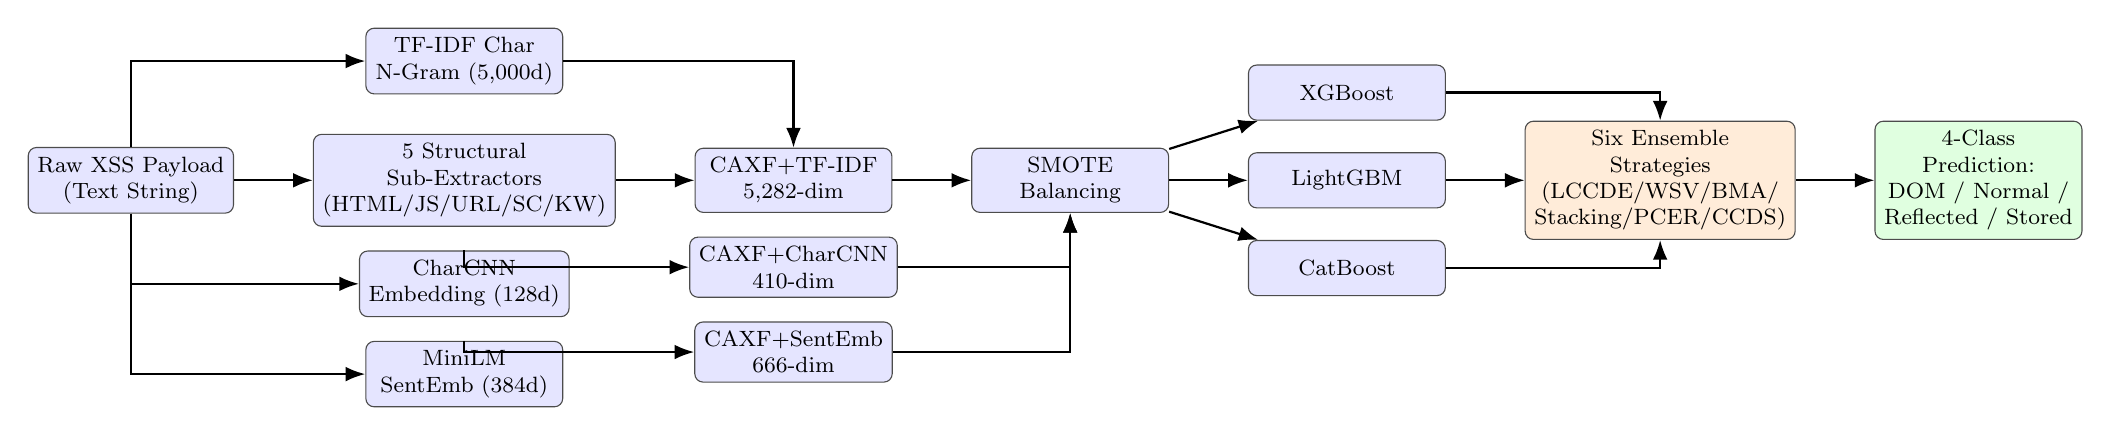
\begin{tikzpicture}[
    node distance = 5mm and 8mm,
    box/.style  = {rectangle, draw=black!70, rounded corners=3pt,
                   fill=blue!10, minimum width=2.5cm, minimum height=7mm,
                   align=center, font=\footnotesize},
    ebox/.style = {rectangle, draw=black!70, rounded corners=3pt,
                   fill=orange!15, minimum width=2.5cm, minimum height=7mm,
                   align=center, font=\footnotesize},
    wbox/.style = {rectangle, draw=black!70, rounded corners=3pt,
                   fill=green!12, minimum width=2.5cm, minimum height=7mm,
                   align=center, font=\footnotesize},
    arr/.style  = {-{Latex[length=2.5mm]}, thick}
  ]
  \node[box] (inp) {Raw XSS Payload\\(Text String)};
  \node[box, right=10mm of inp] (str) {5 Structural\\Sub-Extractors\\(HTML/JS/URL/SC/KW)};
  \node[box, above=5mm of str] (tfidf) {TF-IDF Char\\N-Gram (5,000d)};
  \node[box, below=3mm of str]  (cnn)   {CharCNN\\Embedding (128d)};
  \node[box, below=3mm of cnn]  (mini)  {MiniLM\\SentEmb (384d)};
  \node[box, right=10mm of str] (c1) {CAXF+TF-IDF\\5,282-dim};
  \node[box, below=3mm of c1]   (c2) {CAXF+CharCNN\\410-dim};
  \node[box, below=3mm of c2]   (c3) {CAXF+SentEmb\\666-dim};
  \node[box, right=10mm of c1] (smo) {SMOTE\\Balancing};
  \node[box, right=10mm of smo] (lgbm) {LightGBM};
  \node[box, above=4mm of lgbm] (xgb)  {XGBoost};
  \node[box, below=4mm of lgbm] (cat)  {CatBoost};
  \node[ebox, right=10mm of lgbm] (ens) {Six Ensemble\\Strategies\\(LCCDE/WSV/BMA/\\Stacking/PCER/CCDS)};
  \node[wbox, right=10mm of ens] (out) {4-Class\\Prediction:\\DOM / Normal /\\Reflected / Stored};

  \draw[arr] (inp) -- (str);
  \draw[arr] (inp) |- (tfidf);
  \draw[arr] (inp) |- (cnn);
  \draw[arr] (inp) |- (mini);
  \draw[arr] (str)   -- (c1);
  \draw[arr] (tfidf) -| (c1);
  \draw[arr] (cnn)   |- (c2);
  \draw[arr] (mini)  |- (c3);
  \draw[arr] (c1) -- (smo);
  \draw[arr] (c2) -| (smo);
  \draw[arr] (c3) -| (smo);
  \draw[arr] (smo) -- (xgb);
  \draw[arr] (smo) -- (lgbm);
  \draw[arr] (smo) -- (cat);
  \draw[arr] (xgb)  -| (ens);
  \draw[arr] (lgbm) -- (ens);
  \draw[arr] (cat)  -| (ens);
  \draw[arr] (ens) -- (out);
\end{tikzpicture}
\caption{XSS Sentinel overall pipeline: raw payload $\to$ CAXF feature extraction (three embedding
         backends) $\to$ SMOTE balancing $\to$ three gradient-boosting base classifiers $\to$ six
         ensemble decision strategies $\to$ four-class XSS prediction.}
\label{fig:pipeline}
\end{figure}

%==========================================================================
\section{Conclusion}
\label{sec:conclusion}
%==========================================================================

This section draws together the key outcomes of XSS Sentinel. The conclusion is presented in three
parts. The overall summary consolidates the principal results across all 18 experimental configurations
and places them in the context of the stated objectives from Section~\ref{sec:problem}. The advantages
subsection articulates the properties of the framework that make it practically valuable, tracing
each strength back to a specific design decision in the CAXF pipeline or ensemble architecture. The
limitations subsection provides an honest assessment of the boundaries of the current work---including
statistical constraints imposed by the small DOM-based XSS support, the single-dataset evaluation
scope, inference-cost considerations, and remaining open challenges---so that practitioners can make
informed deployment decisions and researchers can identify the most impactful directions to address next.

\subsection{Overall Summary}

XSS Sentinel demonstrates that combining the CAXF feature extraction pipeline with probabilistic
ensemble decision strategies substantially advances multi-class XSS detection. Across 18 experimental
configurations (6 ensembles $\times$ 3 feature representations), the proposed methods consistently
outperform the LCCDE baseline: Stacking with CAXF+TF-IDF achieves 95.30\% macro-F1 ($+$0.58~pp
over LCCDE); BMA/PCER/WSV with CAXF+SentEmb achieve 99.29\% macro-precision and 95.98\% macro-F1
($+$0.18~pp); Strict LCCDE with OOF leader identification outperforms the heuristic MVE-CT by 1.09~pp
on TF-IDF features. All five proposed ensemble strategies improve upon LCCDE on at least one feature
representation, and the confusion matrices confirm near-perfect classification of Normal and Reflected
XSS across the board, with DOM-based XSS remaining the principal challenge across all configurations.

\subsection{Pros (Advantages)}

XSS Sentinel offers multi-granularity feature fusion through CAXF, simultaneously capturing
structural, syntactic, and semantic payload properties that remain robust to common obfuscation
transforms including HTML entity encoding and JavaScript string splitting. The framework provides
principled ensemble diversity through six complementary decision strategies spanning the full
decision-theory spectrum from hard rule-based LCCDE to Bayesian-probabilistic BMA to meta-learned
Stacking to confidence-adaptive CCDS. Rare-class awareness is built in via SMOTE augmentation and
CatBoost class weighting, ensuring that DOM-based XSS receives meaningful gradient signal even with
only 21 training samples; PCER+CharCNN delivers 99.66\% accuracy with only 0.21\,s inference,
making it immediately production-deployable. All results are fully reproducible with seed=42 from
open data and open-source libraries, with every table value traceable to a specific result file in
the repository's \texttt{results/} directory. The modular architecture means that swapping the CAXF
embedding backend requires only an import-level change while keeping all downstream ensemble logic
identical.

\subsection{Limitations}

The extremely small DOM-based XSS support---21 training and 9 test samples---severely limits the
statistical reliability of DOM F1 comparisons; a single misclassified sample changes DOM F1 by
approximately 0.05, meaning differences of this magnitude should not be over-interpreted. All
experiments are conducted on a single Kaggle dataset, and generalisation to real-world web application
logs containing novel encoding schemes, real WAF bypass payloads, and multi-language scripts has not
been verified. CPU-only MiniLM SentEmb extraction takes 177 to 228 seconds per run, making it
impractical for high-throughput real-time scanning without GPU acceleration. The framework has not
been evaluated against adversarially crafted XSS payloads specifically designed to evade ML-based
detectors. CCDS with CharCNN underperforms the LCCDE baseline (92.60\% vs.\ 94.72\%) due to
JSD-based routing miscalibration in the 410-dim space, requiring threshold re-tuning. Finally, both
BMA and WSV compute their model weights once from training-set statistics and do not adapt to
distributional shift that may occur between training time and deployment.

%==========================================================================
\section{Future Scope}
\label{sec:future}
%==========================================================================

Several directions remain open for extending XSS Sentinel. Adversarial payload augmentation using
grammar-based mutators such as polyglot generators and DOM-Fuzzer would harden the model against
evasion by introducing diverse obfuscation patterns during training beyond what SMOTE alone can
provide. Extending the label set to a five-class schema that includes mutation-based XSS (mXSS)---a
category involving browser-parser quirks not represented in the current four-class benchmark---would
address a growing class of attacks invisible to current WAF rules. Online adaptive ensemble weighting
would replace the static BMA and WSV weights with Bayesian posterior updates that adjust model
influence as new labelled data arrives in a streaming deployment, enabling the framework to gracefully
track concept drift. CCDS threshold calibration via Platt scaling or isotonic regression would
calibrate base-model confidence scores before JSD computation, addressing the
underperformance observed on CharCNN features by ensuring the routing thresholds are appropriate for
each feature space's characteristic disagreement distribution. GPU-accelerated MiniLM inference---using
batched GPU execution---would reduce per-sample extraction from approximately 60\,ms to under 5\,ms,
enabling real-time WAF integration at production traffic volumes. A cross-dataset generalisation study
on benchmarks such as the CSIC HTTP Dataset and real anonymised WAF logs would measure the
transferability of CAXF representations beyond the Kaggle dataset and provide stronger evidence for
deployment readiness. Finally, integrating SHAP or LIME explanations over the CAXF feature dimensions
would identify which structural or n-gram features most strongly indicate each XSS variant, supporting
analyst trust and enabling the semi-automatic generation of interpretable WAF rules from model decisions.

%==========================================================================
\bibliographystyle{plain}
\bibliography{references}
%==========================================================================

\end{document}
